\chapter{Исследование фазовых переходов, магнитных, термодинамических и критических свойств в магнитных спиновых системах}
% \author{Магомедов Магомед Алиевич}
% \date{}

% \begin{document}

% \maketitle

%% \begin{abstract}
%    Методом Ванга-Ландау исследована векторная пятихвершинная модель Поттса на треугольной решетке с учетом конкурирующего обменного взаимодействия между первыми и вторыми ближайшими соседями. Вычислена плотность состояний системы $g(E)$, определены магнитные структуры основного состояния и рассчитаны температурные зависимости различных термодинамических параметров, таких как внутренняя энергия $E$, теплоемкость $C$, энтропия $S$. Показано, что в зависимости от знака обменного взаимодействия между спинами, основное состояние может быть ферромагнитным либо сильно вырожденным.
%% \end{abstract}
%
%\textbf{Целью настоящей работы} является исследование векторной модели Поттса с числом состояний $q=5$ на треугольной решетке методами вычислительной физики.
%
%\textbf{Объектом исследования} являлась векторная модель Поттса с числом состояний $q=5$ на треугольной решетке.
%
%\textbf{Методы исследования.} Для исследования векторной модели Поттса с числом состояний $q=5$ на треугольной решетке нами был разработан комплекс программ для ЭВМ, основанный на алгоритме Ванга-Ландау. Методика исследований, предложенная нами, позволяет не только рассчитать температурные зависимости различных термодинамических параметров, но также определить структуру основного состояния системы, выявить наличие фрустрации или вырождения основного состояния, а также рассчитать энтропию и свободную энергию, что невозможно при использовании других методов. Важной особенностью реализованного нами метода является возможность снятия <<снимка>> основного состояния -- сохранения в графическом файле структуры основного состояния, которая позволяет рассмотреть, какое упорядочение реализуется в системе вблизи абсолютного нуля.

\section{Введение}

Исследование фазовых переходов (ФП), магнитных, термодинамических и критических свойств в магнитных спиновых системах представляет большой теоретический и экспериментальный интерес. Это связано с тем, что для большинства реальных магнитных спиновых систем характерны возмущения различной природы, такие как анизотропия, взаимодействия следующих за ближайшими соседей, внешнее магнитное поле, тепловые и квантовые флуктуации, немагнитные примеси, дефекты, деформации и др. Присутствие этих факторов может повлиять на природу ФП и термодинамические характеристики таких систем \cite{bib:mma-1, bib:mma-2, bib:mma-3, bib:mma-4, bib:mma-5, bib:mma-6, bib:mma-7, bib:mma-8, bib:mma-9, bib:mma-10, bib:mma-11}. Для изучения особенностей термодинамического поведения и природы ФП успешно используются различные решеточные модели. На их основе получено большое количество интересных результатов. Решеточные спиновые модели позволяют описать целый ряд реальных магнитных материалов.

Одной из моделей, применяемых для описания физических систем, является векторная модель Поттса с числом состояний спина $q$. В отчетном году рассматриваются трехкомпонентная модель Поттса на гексагональной решетке, векторная и часовая модели Поттса с числом состояний спина $q=5$ на треугольной решетке. Магнитные материалы на треугольной решетке представляют особый интерес для исследователей. Антиферромагнетики на треугольной решетке представляют собой геометрически фрустрированные спиновые системы, которые исследуются уже давно. Для фрустрированных систем существует совсем немного надежно установленных фактов. Большинство имеющихся результатов получены для модели Изинга, Гейзенберга и Поттса с числом состояний спина $q = 2$, $3$ и $4$.

Многие физические свойства часовой модели зависят от значения $q$. В случае, когда $q = 2$, $3$, $4$, эта модель имеет точное решение. Векторная модель Поттса сводится к модели Изинга и $Z_3$ модели Поттса при $q = 2$ и $3$, соответственно. При $q = 4$ данная модель эквивалентна двум копиям модели Изинга. Установлено, что для этих трех случаев в системе наблюдается ФП второго рода из высокотемпературной парамагнитной фазы в низкотемпературную ферромагнитную упорядоченную фазу. Когда $q \to \infty$ данная векторная модель Поттса сводится к стандартной $XY$ модели. В этом случае спонтанного нарушения симметрии не наблюдается, но происходит ФП из низкотемпературной фазы Березинского-Костерлица-Таулеса в высокотемпературную парамагнитную фазу. Для часовой модели с числом состояний спина $q = 5$ имеется очень мало точно установленных фактов. К настоящему моменту остается открытым вопрос о роде ФП при значении $q = 5$.

Для получения ответа на этот вопрос в данной работе нами проводится исследование двумерной векторной модели Поттса на треугольной решетке с $q = 5$. Исследование этой модели с антиферромагнитными обменными взаимодействиями на треугольной решетке в литературе практически не встречается. Антиферромагнитное обменного взаимодействие в данной модели может привести к фрустрации, вырождению основного состояния, появлению различных фаз и ФП, а также влиять на его термодинамические, магнитные и критические свойства. В связи с этим в данной работе нами предпринята попытка провести исследование ФП и термодинамических свойств этой модели на треугольной решетке.

Исследования проводятся на основе современных методов и идей, что позволит получить ответ на ряд вопросов, связанных с природой ФП и термодинамическим поведением фрустрированных спиновых систем.

\section{Векторная модель Поттса с \texorpdfstring{$q=5$}{q=5} на треугольной решетке и трехкомпонентная модель Поттса на гексагональной решетке}

Модель Поттса была предложена в 1952 году Поттсом по предложению С. Домба. Модель задается числом состояний $q$, в которых может находиться спин на произвольной решетке.

Гамильтониан векторной модели Поттса с числом состояний $q=5$ на треугольной решетке может быть представлен в следующем виде:
\begin{equation*}
    H = -J \sum_{i, j} \cos \left(\theta_i - \theta_J\right),
\end{equation*}
где спиновые состояния $q$ в узле $i$ обозначены плоским углом $\theta_i = 2\pi k/q$, $k = 1, \dots, q$. В данном исследовании нами рассматриваются два случая. В первом случае $J > 0$ -- параметр ферромагнитного обменного взаимодействия, а во втором случае $J < 0$ -- параметр антиферромагнитного обменного взаимодействия.

%\section{Трехкомпонентная модель Поттса на гексагональной решетке} 

Приведем также гамильтониан трехкомпонентной модели Поттса c числом состояний спина $q=3$ на гексагональной решетке. Он может быть представлен в следующем виде \cite{bib:bab-8, bib:bab-9}:
\begin{equation*}
    H = -\frac{1}{2} J \sum_{i, j} \delta(S_i, S_j), \quad S_i = P_1, P_2, P_3
\end{equation*}
где $J$ -- параметр ферромагнитного ($J>0$) взаимодействия ближайших спинов, $P_i$ число состояний выбранного спина $S_i$. Из аналитических теорий известно, что в двумерных моделях Поттса с числом состояний спина $q=3$ и $q=4$ в однородном состоянии наблюдается ФП второго рода. К настоящему времени критическое поведение этих моделей на различных решетках не изучено достаточно хорошо.

%Все исследования, проведены с использованием высокоэффективного кластерного алгоритма Вольфа \cite{bib:bab-10} метода Монте-Карло (МК). Расчеты проводились для систем с периодическими граничными условиями. Исследовались системы с линейными размерами $L=10 - 320$. Для вывода системы в равновесное состояние вычислялось время релаксации $\tau_0$ соответствующее для каждой системы с линейными размерами $L$. Этот неравновесный участок отбрасывали. Кроме того, усреднение проводилось по участку марковской цепи длиной $\tau=400\tau_0$. Причем, для самой большой системы $L=320$, $\tau_0 = 2 \times 10^4$ МК шагов/спин.


%\section{Метод исследований}
%
%Исследования проводились на основе алгоритма Ванга-Ландау метода Монте-Карло (МК) \cite{bib:mma-9,bib:mma-10,bib:mma-11}. Данный алгоритм является реализацией метода энтропийного моделирования и его основной особенностью является возможность расчета функции плотности состояний системы, зная которую можно легко вычислить любые интересующие нас термодинамические параметры системы.
%
%Алгоритм Ванга-Ландау является разновидностью энтропийного моделирования и, как показывает опыт его применения в последние годы, является весьма эффективным для исследования различных дискретных спиновых систем \cite{bib:mma-9}.
%
%Алгоритм Ванга-Ландау основан на том, что совершая случайное блуждание в пространстве энергий с вероятностями, обратно пропорциональными плотности состояний $g(E)$, мы получаем равномерное распределение по энергиям. Подобрав вероятности перехода такими, что посещение всех энергетических состояний стало бы равномерным, можно получить изначально неизвестную плотность состояний $g(E)$, зная которую можно вычислить значения необходимых термодинамических параметров при любой температуре. Так как плотность состояний $g(E)$ очень быстро растет с увеличением размеров исследуемых систем, для удобства хранения и обработки больших чисел пользуются величиной $\ln g(E)$.
%
%Важным обстоятельством является то, что плотность состояний $g(E)$ не зависит от температуры, следовательно, рассчитав ее однократно, мы можем вычислить значения любых термодинамических параметров системы при любой ненулевой температуре.
%
%В данной работе нами алгоритм Ванга-Ландау был использован в следующем виде \cite{bib:mma-9,bib:mma-10,bib:mma-11}:
%\begin{itemize}
%    \item Задается произвольная начальная конфигурация спинов. Стартовые значения плотности состояний $g(E)=1$, гистограммы распределений по энергиям $H(E)=1$ и начальное значение модификационного фактора $f = f_0 = e^1 \approx 2.71828$.
%    \item Многократно совершаем шаги в фазовом пространстве, пока не получим относительно плоскую гистограмму $H(E)$ (т.е. пока не будут посещены примерно одинаковое количество раз все возможные энергетические состояния системы). В качестве критерия <<плоскости>> гистограммы нами принималось условие отклонения числа посещений всех возможных (с ненулевой плотностью $g(E) \neq 1$) энергетических состояний на величину не более чем на 10\% от среднего значения по системе.
%    \item При этом вероятность перехода из состояния с энергией $E_1$ в состояние с энергией $E_2$ определяется по формуле $p = g(E_1) / g(E_2)$. Если переход в состояние с энергией $E_2$ состоялся, то для энергии $E_2$ проводится модификация плотности состояния $g(E_2) \to f \times g(E_2)$, и гистограммы $H(E_2) \to H(E_2) + 1$ иначе меняем параметры для энергии $E_1$ $g(E_1) \to f \times g(E_1)$ $H(E_1) \to H(E_1) + 1$.
%    \item Если гистограмма стала <<плоской>>" то: обнуляем гистограмму $H(E) \to 0$,  уменьшаем модификационный фактор $f \to \sqrt{f}$, и продолжаем снова и снова, пока модификационный фактор $f \geq f_{\min}$. В качестве минимального значения модификационного фактора нами принималось $f_{\min} = 1.0000000001$.
%    \item Каждый раз при достижении энергетического минимума нами проводился анализ магнитной структуры основного состояния и его запись в графический файл. При этом проводилось сравнение полученной конфигурации с ранее полученными и только при обнаружении новой уникальной конфигурации производится ее сохранение в графический файл. Далее данная структура заносится в специальную базу данных для данной модели для дальнейшего сравнения. Данная процедура позволяет избежать дублирования в графических файлах многократно встречающихся состояний с одинаковой магнитной структурой.
%    \item После расчета плотности состояний системы для любой интересующей нас температуры рассчитываются различные термодинамические параметры, такие как, энтропия, внутренняя энергия, свободная энергия, теплоемкость, намагниченность, восприимчивость и т.д.
%\end{itemize}
%
%Более подробно алгоритм Ванга-Ландау изложен в работах \cite{bib:mma-9,bib:mma-10,bib:mma-11}.
\section{Результаты}
%\subsection{Векторная пятихвершинная модель Поттса на треугольной решетке}
%\subsection{ММА}
Начнем с результатов исследования векторной модели Поттса на треугольной решетке методом Ванга--Ландау \cite{bib:mma-9, bib:mma-10, bib:mma-11}.
На рис.~\ref{fig:mma-2} даны плотности состояний $g(E)$ для разных линейных размеров системы для ферромагнитной и антиферромагнитной моделей (здесь и далее статистическая погрешность не превышает размеров символов, использованных для построения зависимостей). Как видно на рисунке, плотность состояний имеет куполообразную форму. С увеличением линейных размеров системы максимум плотности состояний $g(E)$ значительно возрастает.
\begin{figure}[ht]
    \centering
    \begin{subfigure}{0.45\textwidth}
        \includegraphics[width=0.9\linewidth]{mma/image17.png}
        \caption{для ферромагнитной модели;}
    \end{subfigure}
    \begin{subfigure}{0.45\textwidth}
        \includegraphics[width=0.9\linewidth]{mma/image18.png}
        \caption{для антиферромагнитной модели;}
    \end{subfigure}
    \caption{Плотность состояний $g(E)$ при различных линейных размерах $L$.}
    \label{fig:mma-2}
\end{figure}

На рис.~\ref{fig:mma-3}. представлены характерные зависимости теплоемкости $C$ от температуры для ферромагнитной и антиферромагнитной моделей с различными линейными размерами системы $L$. Отметим, что для ферромагнитной модели (рис.~\ref{fig:mma-3a}) на зависимостях теплоемкости $C$ от температуры для всех систем вблизи критической температуры наблюдаются два хорошо выраженных максимума. Наличие двух максимумов на температурной зависимости теплоемкости позволяет говорить о двух последовательных ФП в данной модели.
\begin{figure}[ht]
    \centering
    \begin{subfigure}{0.45\textwidth}
        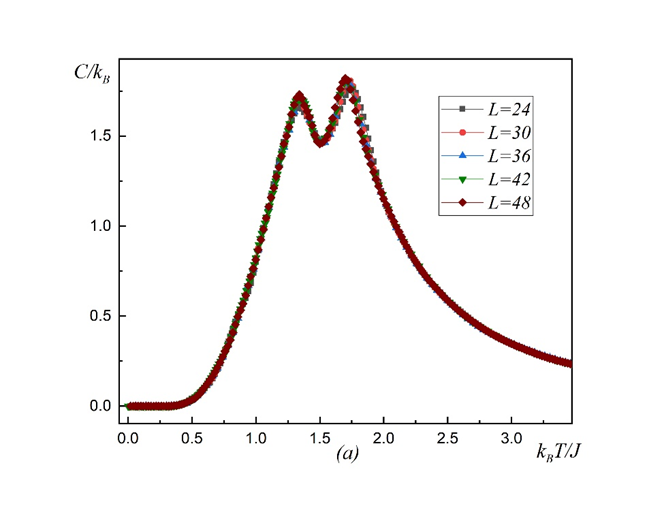
\includegraphics[width=0.9\linewidth]{mma/image19.png}
        \caption{для ферромагнитной модели;}
        \label{fig:mma-3a}
    \end{subfigure}
    \begin{subfigure}{0.45\textwidth}
        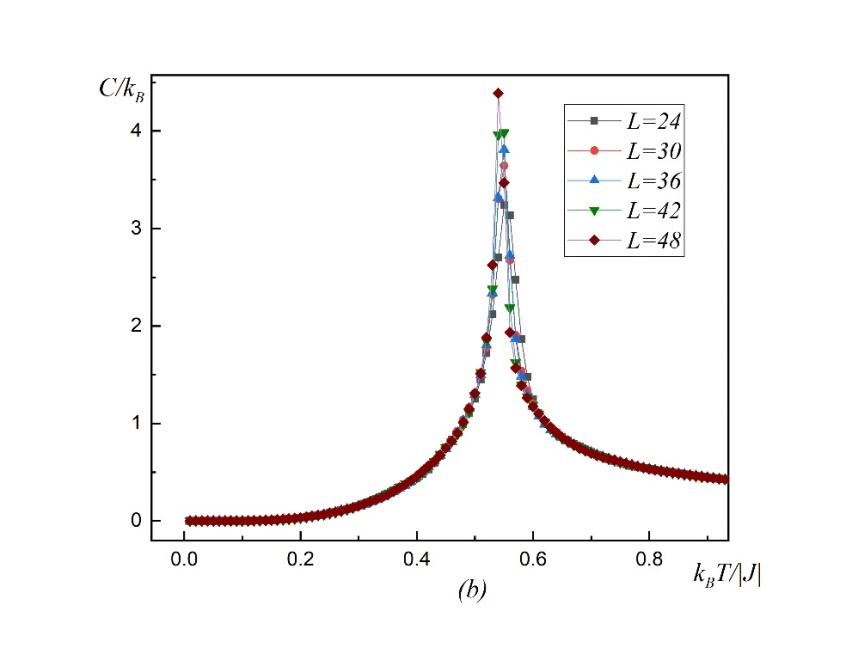
\includegraphics[width=0.9\linewidth]{mma/image20.jpeg}
        \caption{для антиферромагнитной модели;}
        \label{fig:mma-3b}
    \end{subfigure}
    \caption{Зависимость теплоемкости $C/k_B$ от температуры $k_B T/ \left|J\right|$ для разных $L$.}
    \label{fig:mma-3}
\end{figure}

\begin{figure}[ht]
    \begin{subfigure}{0.33\textwidth}
        
\includegraphics[width=0.9\linewidth]{mma/image21.png}
        \caption{в интервале температур $0 \leq T < Tc_1$;}
        \label{fig:mma-4a}
    \end{subfigure}
    \begin{subfigure}{0.33\textwidth}
        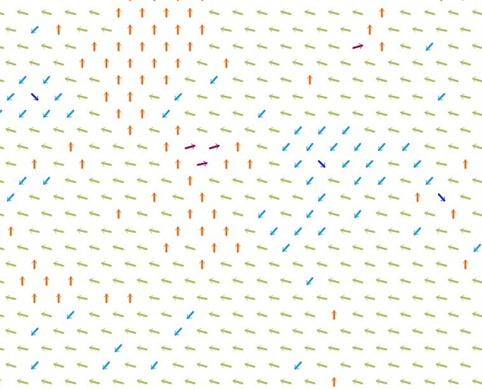
\includegraphics[width=0.9\linewidth]{mma/image22.png}
        \caption{в интервале температур $Tc_1 < T < Tc_2$;}
        \label{fig:mma-4b}
    \end{subfigure}
    \begin{subfigure}{0.33\textwidth}
        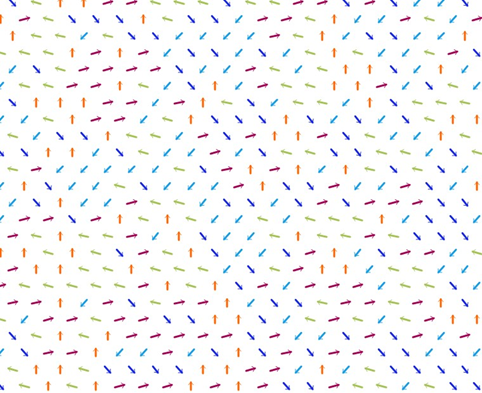
\includegraphics[width=0.9\linewidth]{mma/image23.png}
        \caption{$T > Tc_2$;}
        \label{fig:mma-4c}
    \end{subfigure}
    \caption{Магнитные структуры основного состояния для ферромагнитной модели;}
    \label{fig:mma-4}
\end{figure}

Для антиферромагнитной модели (рис.~\ref{fig:mma-3b}) наблюдается только один максимум, что позволяет говорить об одном ФП. Все максимумы увеличиваются с ростом числа спинов в системе, причем они в пределах погрешности приходятся на одну и ту же температуру даже для систем с наименьшим значением $L$. Это свидетельствует, во-первых, о высокой эффективности использованного способа добавления периодических граничных условий, а во-вторых, о достижении насыщения по $N$ для многих исследуемых нами параметров.

Для определения типа упорядочения нами проведен анализ магнитных структур основного состояния в широком температурном интервале. На рис.~\ref{fig:mma-4} приведены полученные нами структуры. На рисунке видно, что в данной модели наблюдаются три типа магнитного упорядочения: в интервале температур $0 \leq T < Tc_1$ (рис.~\ref{fig:mma-4a}) наблюдается полностью упорядоченная ферромагнитная фаза; в интервале $Tc_1 < T < Tc_2$ (рис.~\ref{fig:mma-4b}) -- фаза типа Березинского-Костерлица-Таулеса, где наблюдается ближний порядок в системе, в котором превалирует одно из пяти состояний спина; при дальнейшем повышении температуры $T > Tc2$ (рис.~\ref{fig:mma-4c}) -- полностью разупорядоченная парамагнитная фаза.

\begin{figure}[ht]
    \centering
    \begin{subfigure}{0.45\textwidth}
        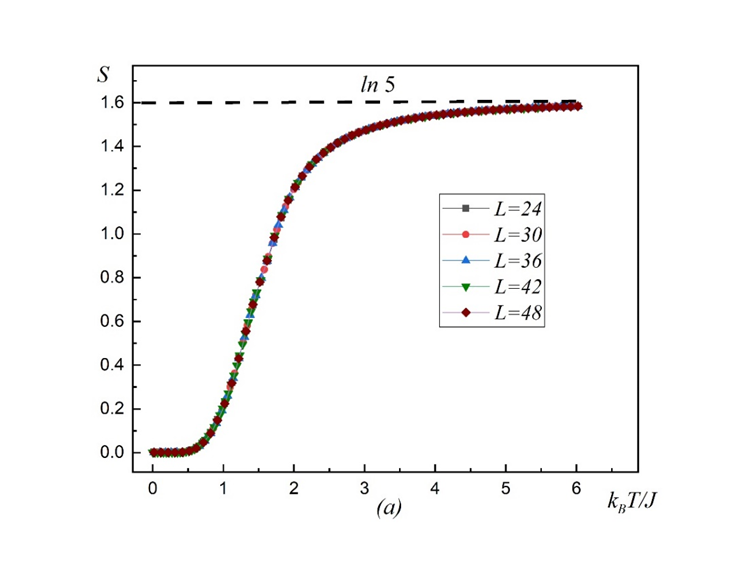
\includegraphics[width=0.9\linewidth]{mma/image24.png}
        \caption{для ферромагнитной модели;}
    \end{subfigure}
    \begin{subfigure}{0.45\textwidth}
        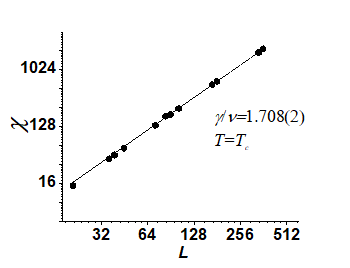
\includegraphics[width=0.9\linewidth]{mma/image25.png}
        \caption{для антиферромагнитной модели;}
    \end{subfigure}
    \caption{Температурные зависимости энтропии $S$.}
    \label{fig:mma-5}
\end{figure}

На рис.~\ref{fig:mma-5} приведены температурные зависимости энтропии $S$ для обоих моделей. Из рисунков видно, что с увеличением температуры энтропия для всех систем стремится к теоретически предсказанному значению $\ln 5$. При низких температурах, близких к абсолютному нулю, для ферромагнитной модели энтропия стремится к нулевому значению для всех значений $L$. Нулевая остаточная энтропия свидетельствует об отсутствии вырождения основного состояния. Для антиферромагнитной модели энтропия при низких температурах стремится к ненулевому значению для всех значений $L$. Такое поведение свидетельствует о сильном вырождении данной модели, что также характерно для фрустрированных систем.

Для анализа характера ФП использовался метод кумулянтов Биндера четвертого порядка по энергии, который имеет следующий вид:
\begin{equation*}
    V_L (T) = 1 - \frac{\left<E^4\right>}{\left<E^2\right>^2}
\end{equation*}

Известно, что ФП второго рода характеризуются следующими отличительными особенностями: усредненная величина $V_L (T)$ стремится к тривиальному значению согласно выражению $V_L (T) = V* + b L^{-d}$ при $L \to \infty$ и $T = T(L)$, где $V* = 2/3$.

Характерные зависимости кумулянтов Биндера $V_L(T)$ от температуры для систем с линейными размерами для ферромагнтной и антиферромагнитной моделей приведены на рис.~\ref{fig:mma-6}. Как видим из рисунков энергетические кумулянты для обоих моделей показывают разный характер поведения. Для антиферромагнитного случая на графиках зависимости энергетических кумулянтов наблюдаются минимумы в области температуры фазового перехода, которые уменьшаются с увеличением размеров системы $L$. Для ферромагнитной модели такие минимумы не наблюдаются. Заметим, что на вставке к рис.~\ref{fig:mma-6b} наглядно видно, что тривиальная величина $V* \to 2/3$ при $L \to \infty$. Такое поведение, как отмечалось выше, характерно для ФП второго рода.
\begin{figure}[ht]
    \centering
    \begin{subfigure}{0.45\textwidth}
        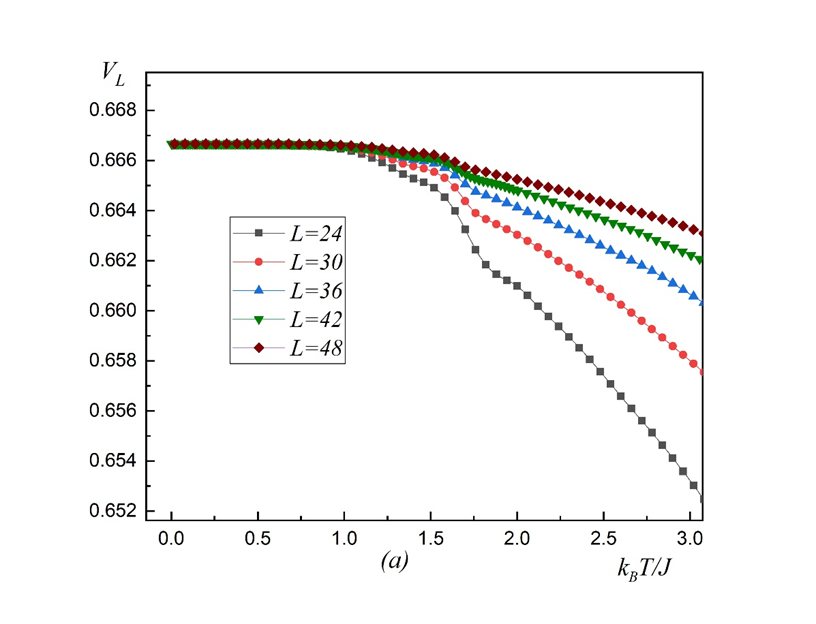
\includegraphics[width=0.9\linewidth]{mma/image27.png}
        \caption{для ферромагнитной модели;}
        \label{fig:mma-6a}
    \end{subfigure}
    \begin{subfigure}{0.45\textwidth}
        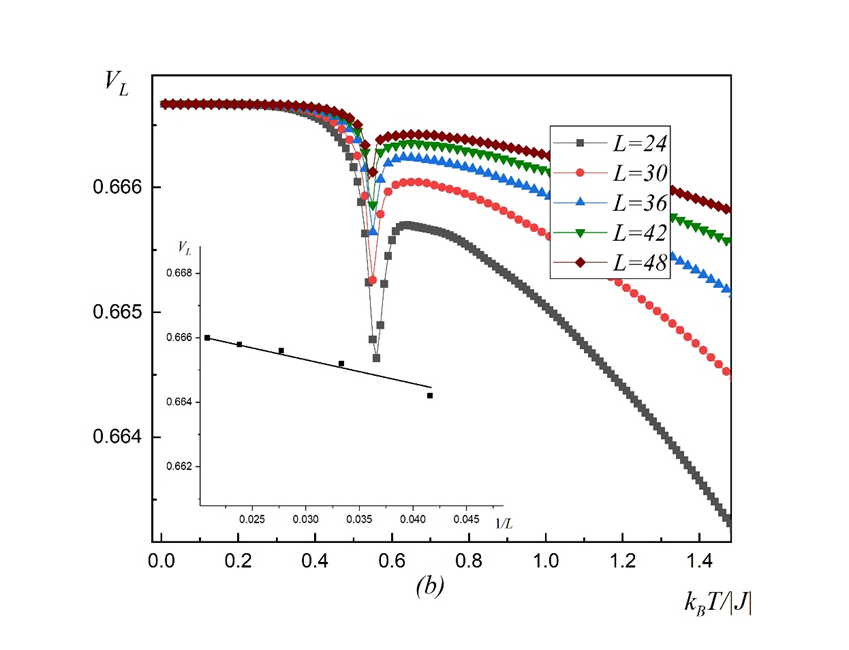
\includegraphics[width=0.9\linewidth]{mma/image28.png}
        \caption{для антиферромагнитной модели;}
        \label{fig:mma-6b}
    \end{subfigure}
    \caption{Температурная зависимость кумулянтов Биндера $V_L (T)$.}
    \label{fig:mma-6}
\end{figure}

Для более точного определения рода ФП мы использовали гистограммный анализ данных метода МК. В случае ФП первого рода на гистограмме распределения энергии вблизи температуры перехода наблюдается бимодальное распределение энергии. То есть, на графике появляются два максимума, расположенных симметрично относительно равновесного значения энергии. В случае ФП второго рода должен наблюдаться один максимум.

\begin{figure}[ht]
    \centering
    \begin{subfigure}{0.45\textwidth}
        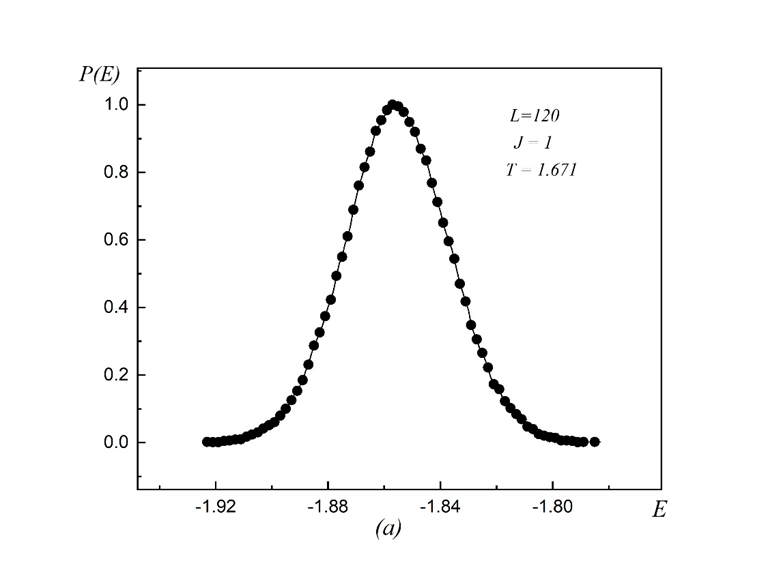
\includegraphics[width=0.9\linewidth]{mma/image29.png}
        \caption{для ферромагнитной модели;}
        \label{fig:mma-7a}
    \end{subfigure}
    \begin{subfigure}{0.45\textwidth}
        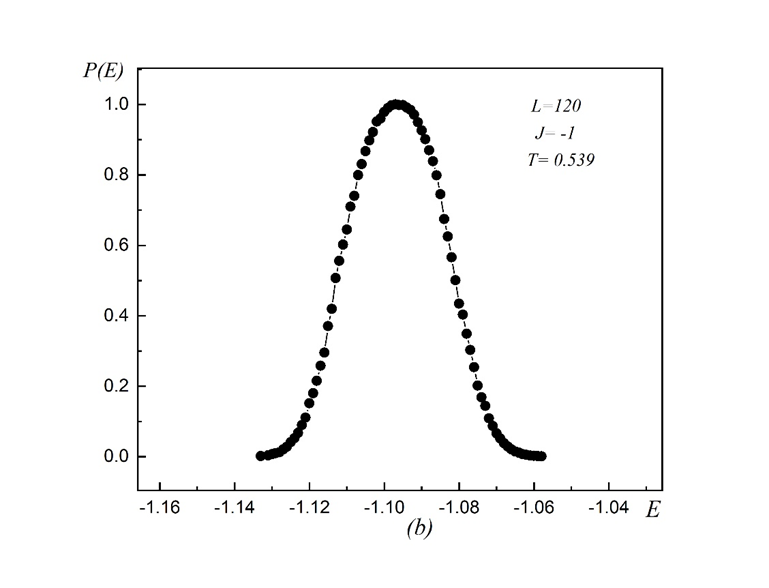
\includegraphics[width=0.9\linewidth]{mma/image30.png}
        \caption{для антиферромагнитной модели;}
        \label{fig:mma-7b}
    \end{subfigure}
    \caption{Гистограмма распределения энергии.}
    \label{fig:mma-7}
\end{figure}

На рис.~\ref{fig:mma-7a} и \ref{fig:mma-7b} представлены гистограммы распределения энергии для линейных размеров системы $L =120$ в области температуры ФП для ферромагнитной и антиферромагнитной моделей. На графиках зависимости вероятности $P$ от энергии системы $E$ наблюдается один хорошо выраженный максимум, который свидетельствует о наличии в антиферромагнитной модели ФП второго рода. Для ферромагнитной часовой модели подобный анализ показывает наличие одного максимума, который позволяет нам утверждать, что в данной модели точно не наблюдается ФП первого рода. Такое поведение характерно для ФП второго рода. Однако, анализ магнитных структур основного состояния свидетельствует в пользу перехода типа Березинского-Костерлица-Таулеса (рис.~\ref{fig:mma-4}). 

%\subsection{Исследование фазовых переходов и термодинамических свойств часовой модели с числом состояний спина \texorpdfstring{$q = 5$}{q=5}}

% \begin{abstract}
%    С помощью алгоритма Ванга-Ландау метода Монте-Карло проведены исследования фазовых переходов и термодинамических свойств часовой модели с числом состояний спина $q = 5$ на треугольной решетке. Используя гистограммный метод проведен анализ фазовых переходов. Показано, что в ферромагнитной часовой модели наблюдаются два фазовых перехода типа Березинского-Костерлица-Таулеса, а в антиферромагнитной часовой модели обнаружен фазовый переход второго рода.
% \end{abstract}

%\section*{Введение}
%
%Исследование фазовых переходов (ФП), магнитных, термодинамических и критических свойств в магнитных спиновых системах представляет большой теоретический и экспериментальный интерес. Это связано с тем, что для большинства реальных магнитных спиновых систем характерны возмущения различной природы, такие как анизотропия, взаимодействия следующих за ближайшими соседей, внешнее магнитное поле, тепловые и квантовые флуктуации, немагнитные примеси, дефекты, деформации и др. Присутствие этих факторов может повлиять на природу ФП и термодинамические характеристики таких систем \cite{bib:rmk-1, bib:rmk-2, bib:rmk-3}. Для изучения особенностей термодинамического поведения и природы ФП успешно используются различные решеточные модели. На их основе получено большое количество интересных результатов. Решеточные спиновые модели позволяют описать целый ряд реальных магнитных материалов.
%
%Одной из моделей, применяемых для описания физических систем, является часовая модель с числом состояний спина $q$. Нами в данном исследовании рассматривается часовая модель с числом состояний спина $q=5$ на треугольной решетке. Магнитные материалы на треугольной решетке представляют особый интерес для исследователей. Антиферромагнетики на треугольной решетке представляют собой геометрически фрустрированные спиновые системы, которые исследуются уже давно. Для фрустрированных систем существует совсем немного надежно установленных фактов. Большинство имеющихся результатов получены для модели Изинга, Гейзенберга и Поттса с числом состояний спина $q = 2$, $3$ и $4$ \cite{bib:rmk-4, bib:rmk-5, bib:rmk-6}.
%
%Многие физические свойства часовой модели зависят от значения $q$. В случае, когда $q = 2$, $3$, $4$, эта модель имеет точное решение. Установлено, что для этих трех случаев в системе наблюдается ФП второго рода из высокотемпературной парамагнитной фазы в низкотемпературную ферромагнитную упорядоченную фазу. Когда $q \to \infty$ данная модель сводится к стандартной $XY$ модели. В этом случае спонтанного нарушения симметрии не наблюдается, но происходит ФП из низкотемпературной фазы Березинского-Костерлица-Таулеса (БКТ) в высокотемпературную парамагнитную фазу. Для часовой модели с числом состояний спина $q = 5$ имеется очень мало точно установленных фактов. К настоящему моменту остается открытым вопрос о роде ФП при значении $q = 5$.
%
%Для получения ответа на этот вопрос в данной работе нами проводится исследование двумерной часовой модели на треугольной решетке с $q = 5$. Исследование этой модели с антиферромагнитными обменными взаимодействиями на треугольной решетке в литературе практически не встречается. Антиферромагнитное обменного взаимодействие в данной модели может привести к фрустрации, вырождению основного состояния, появлению различных фаз и ФП, а также влиять на его термодинамические, магнитные и критические свойства. В связи с этим в данной работе нами предпринята попытка провести исследование ФП и термодинамических свойств этой модели на треугольной решетке.
%
%Исследования проводятся на основе современных методов и идей, что позволит получить ответ на ряд вопросов, связанных с природой ФП и термодинамическим поведением фрустрированных спиновых систем.
%
%\section*{Результат исследования}

%\subsection{РМК}
Перейдем теперь к результатам, относящимся к часовой модели с числом состояний спина $q = 5$. На рис.~\ref{fig:rmk-1} приведены температурные зависимости энтропии $S$, полученные с помощью алгоритма Ванга-Ландау метода Монте-Карло.

\begin{figure}[ht]
    \centering
    \begin{subfigure}{0.45\textwidth}
        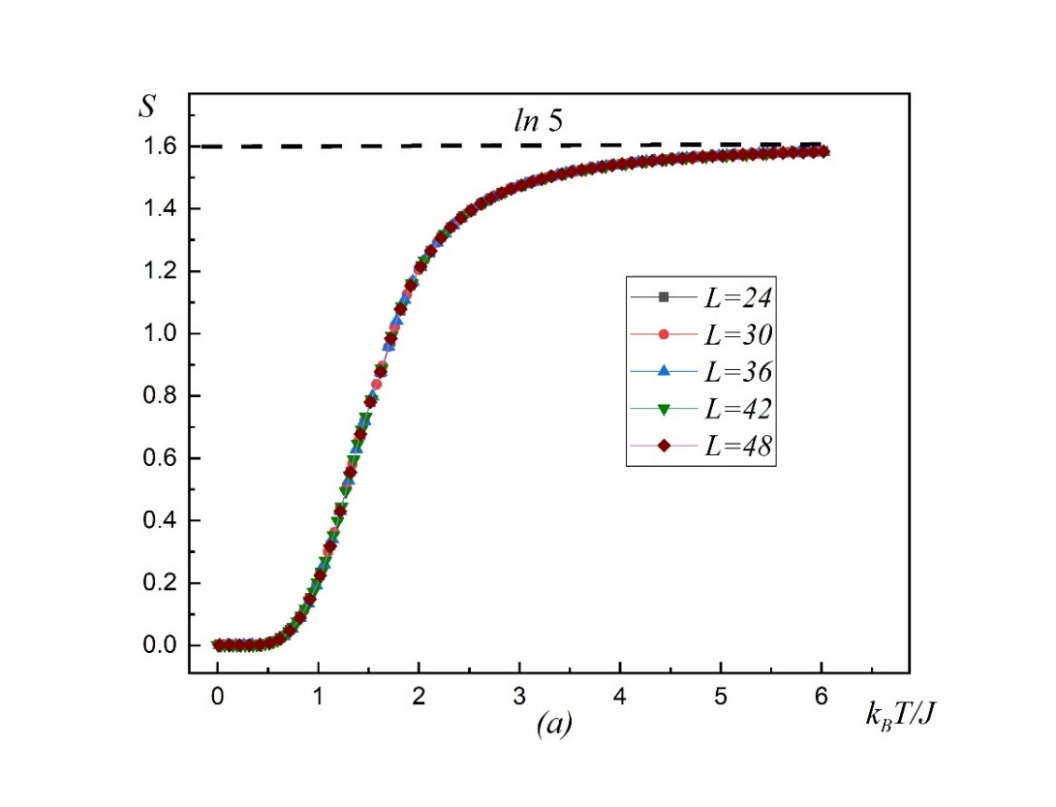
\includegraphics[width=\linewidth]{rmk/image1.jpeg}
        \caption{}
    \end{subfigure}
    \begin{subfigure}{0.45\textwidth}
        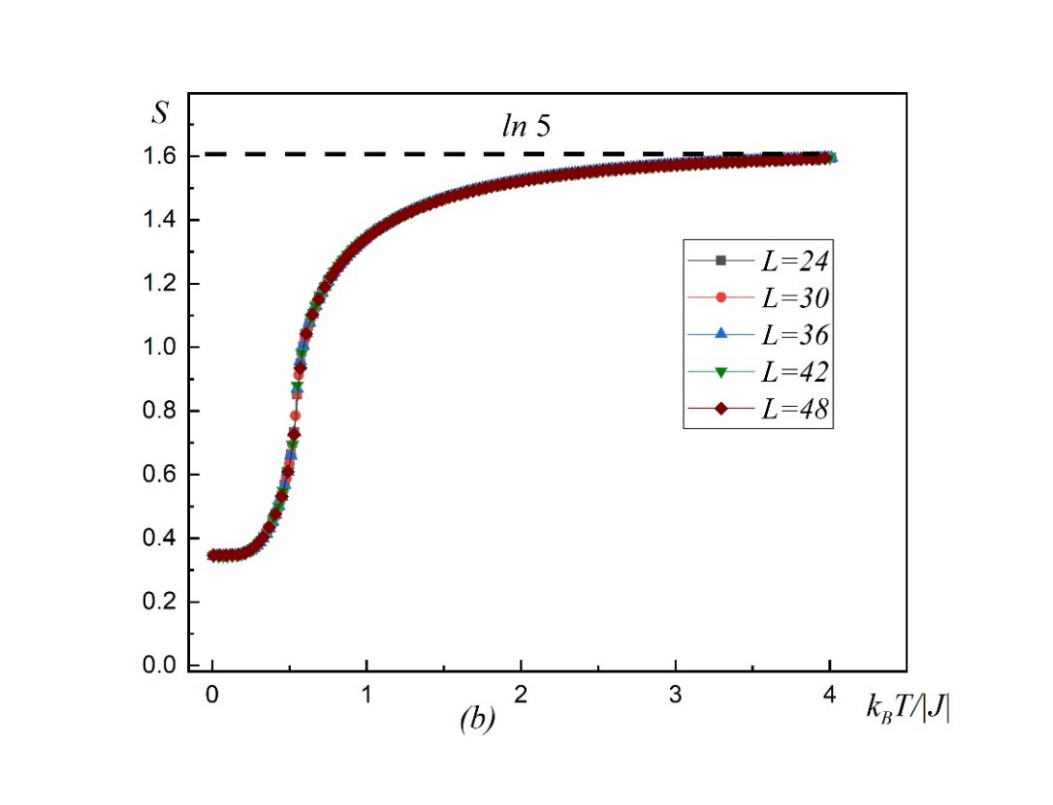
\includegraphics[width=\linewidth]{rmk/image2.jpeg}
        \caption{}
    \end{subfigure}
    \caption{Температурные зависимости энтропии S. a) для ферромагнитной модели; b) для антиферромагнитной модели.}
    \label{fig:rmk-1}
\end{figure}

Из рисунков видно, что с увеличением температуры энтропия для всех систем стремится к теоретически предсказанному значению $\ln 5$. При низких температурах, близких к абсолютному нулю, для ферромагнитной модели энтропия стремится к нулевому значению для всех значений $L$. Нулевая остаточная энтропия свидетельствует об отсутствии вырождения основного состояния. Для антиферромагнитной модели энтропия при низких температурах стремится к ненулевому значению для всех значений $L$. Такое поведение свидетельствует о сильном вырождении данной модели, что характерно для фрустрированных систем.

\begin{figure}[ht]
    \centering
    \begin{subfigure}{0.45\textwidth}
        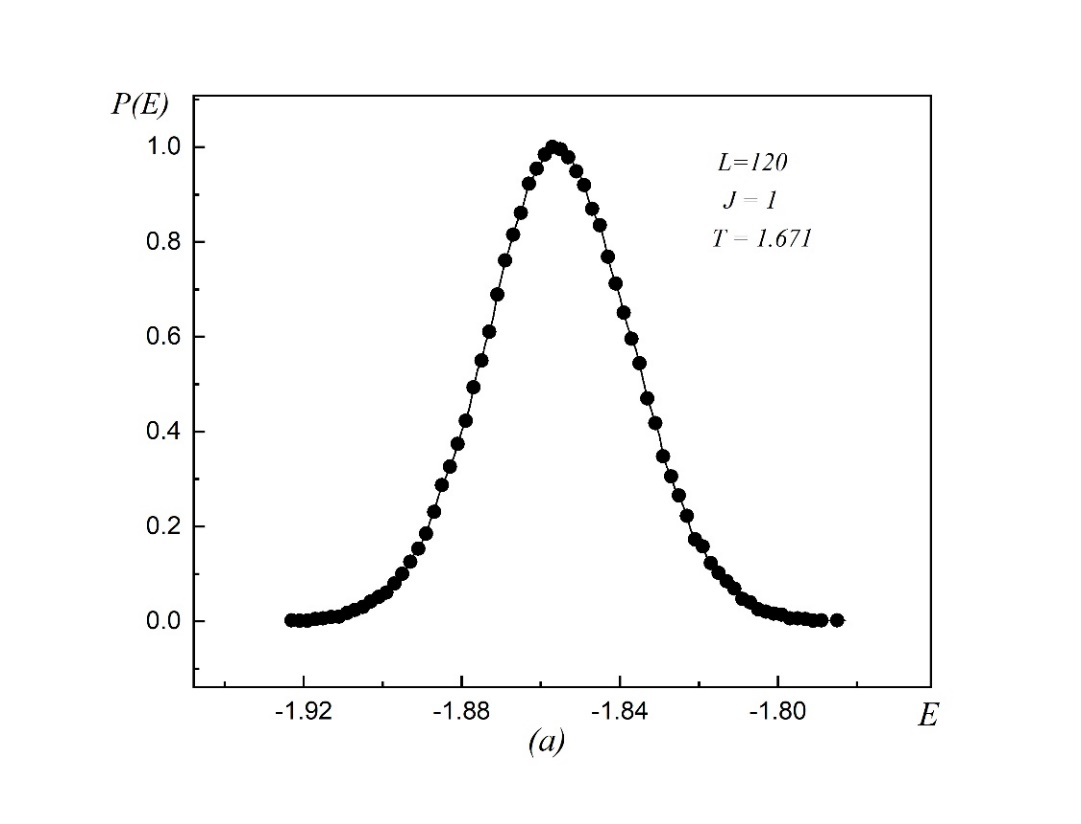
\includegraphics[width=\linewidth]{rmk/image3.jpeg}
        \caption{}
        \label{fig:rmk-2:a}
    \end{subfigure}
    \begin{subfigure}{0.45\textwidth}
        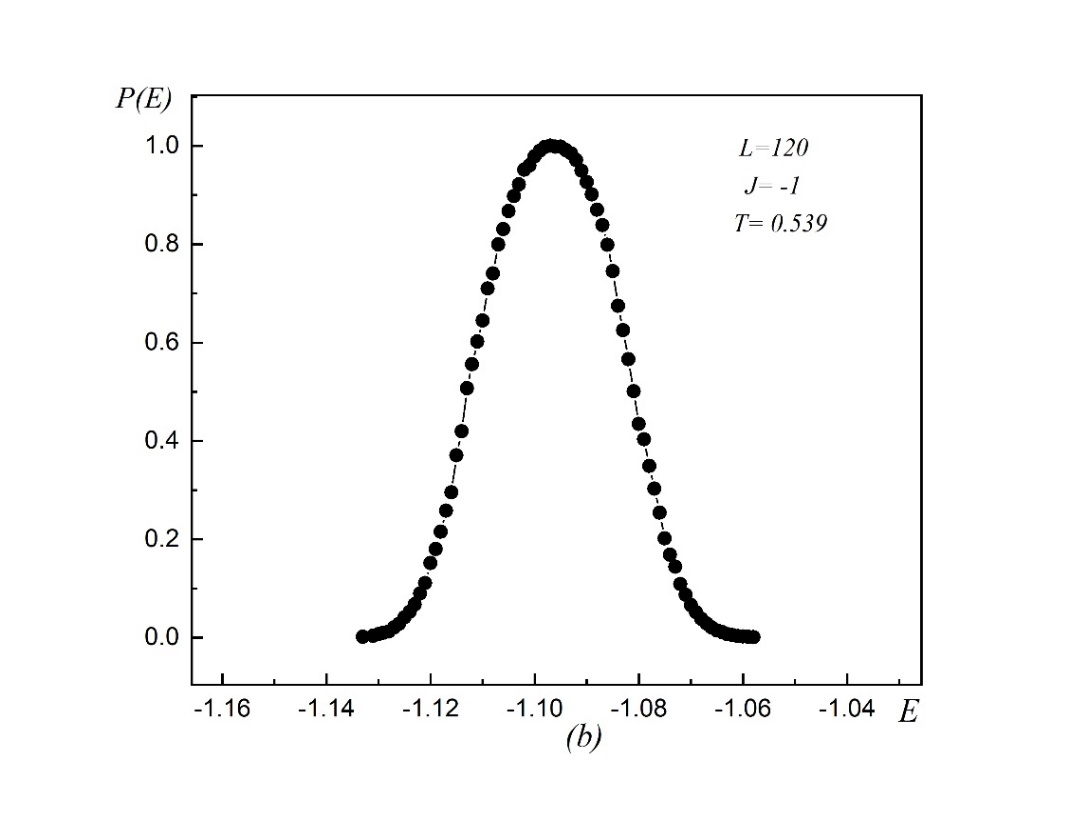
\includegraphics[width=\linewidth]{rmk/image4.jpeg}
        \caption{}
        \label{fig:rmk-2:b}
    \end{subfigure}
    \caption{Гистограмма распределения энергии. a) для ферромагнитной модели; b) для антиферромагнитной модели.}
    \label{fig:rmk-2}
\end{figure}

Для определения рода ФП мы использовали гистограммный анализ данных метода Монте-Карло. В случае ФП первого рода на гистограмме распределения энергии вблизи температуры перехода наблюдается бимодальное распределение энергии. То есть, на графике появляются два максимума, расположенных симметрично относительно равновесного значения энергии. В случае ФП второго рода должен наблюдаться один максимум. На рис.~\ref{fig:rmk-2:a} и \ref{fig:rmk-2:b} представлены гистограммы распределения энергии для линейных размеров системы $L=120$ в области температуры ФП для ферромагнитной и антиферромагнитной моделей. На графиках зависимости вероятности $P$ от энергии системы $E$ наблюдается один хорошо выраженный максимум, который свидетельствует о наличии в антиферромагнитной модели ФП второго рода. Для ферромагнитной часовой модели подобный анализ показывает наличие одного максимума, который позволяет нам утверждать, что в данной модели точно не наблюдается ФП первого рода. Такое поведение характерно для ФП второго рода.

%\chapter{Исследование фазового перехода и критического поведения в модели Поттса с числом состояний спина \texorpdfstring{$q=3$}{q=3} на гексагональной решетке методом Монте-Карло}

%\subsubsection*{Ключевые слова}
%
%Модель Поттса, фазовые переходы, критическое поведение
%
%\subsubsection*{Реферат}
%
%Объектом исследования является модель Поттса с числом состояний спина $q=3$ на гексагональной решетке. Целью НИР является: исследование фазового перехода и критического поведения в двумерной трехкомпонентной ($q=3$) модели Поттса на гексагональной решетке;
%
%\paragraph*{Методы численного эксперимента:}
%
%Метод Монте-Карло (кластерный алгоритм Вольфа).
%
%\subsubsection*{Полученные результаты:}
%
%С применением численных методов Монте-Карло показано, что в модели Поттса с числом состояний спина $q=3$ на гексагональной решетке наблюдается фазовый переход второго рода с критическими показателями соответствующие классу универсальности трехкомпонентной модели Поттса.

% Основная часть

%\section{Введение}
%
%В физике конденсированных сред огромный интерес вызывают как фазовые переходы (ФП), так и связанные с ними критические явления в чистых и разбавленных спиновых системах. На разработку эффективной теории ФП и КЯ были затрачены колоссальные усилия и к настоящему моменту времени в этом направлении достигнут существенный прогресс. Создание теории Л.Д. Ландау и разработка флуктуационной теории фазовых переходов \cite{bib:bab-1}, идеи, заложенные в теории ренормализационной группы и \varepsilon-разложения \cite{bib:bab-2, bib:bab-3, bib:bab-4}, предложенные Вильсоном, а также применение гипотезы подобия (скейлинг), основы которой были заложены в 60-х годах \cite{bib:bab-1, bib:bab-5}, с последующим решением большого количества технических вопросов, позволили достичь колоссального прогресса в понимании процессов, происходящих при ФП. Кроме того, развит мощный математический аппарат, оказавшийся полезным не только для теории критических явлений, но и ряда весьма далеких от нее областей физики.
%
%Существенный вклад в строгую количественную теорию кооперативных явлений в спиновых системах внесли также методы высоко- и низкотемпературных разложений \cite{bib:bab-6, bib:bab-7}. Было показано, что критические индексы (КИ) не зависят от величины спина, а если и зависят, то настолько слабо, что этой зависимостью даже в хорошем приближении можно пренебречь \cite{bib:bab-6}. Полученные закономерности позволили сформулировать гипотезу универсальности для статического критического поведения: критическое поведение (КП) зависит от размерности пространства (решетки), топологии параметра порядка, симметрии гамильтониана, радиуса характерного взаимодействия.
%
%Из этой гипотезы следует, что в рамках одного класса универсальности для всех спиновых систем, испытывающих фазовый переход второго рода, критические индексы являются одинаковыми. В один и тот же класс универсальности попадают, столь непохожие на первый взгляд, системы как жидкости, магнетики, сегнетоэлектрики, сверхпроводники и другие. Следует отметить, что теоретические исследования показывают, что в двумерных моделях Поттса фазовый переход будет первого рода (со скрытой теплотой перехода), когда $q>4$ и непрерывным (без скрытой теплоты) при $q\leq4$. Результаты теоретических исследований \cite{bib:bab-8, bib:bab-9} ничего не говорят о том, каковы критические показатели при $q\leq4$. Это связано с тем, что теоретические подходы при рассмотрении модели Поттса сталкиваются с большими и труднопреодолимыми проблемами. Двумерная модель Поттса с $q=3$ и $q=4$ до настоящего времени не решена точно. Изучение магнитных и тепловых свойств в этих моделях в чистом и разбавленном (немагнитной примесью) режиме на различных двумерных решетках имеет важное фундаментальное и прикладное значение и их исследование к настоящему времени является своевременным.



%\subsection{БАБ}
Ниже приведены результаты, полученные для трехкомпонентной модели на гексагональной решетке.
Наблюдение за температурным ходом энергии $U$, намагниченности $m$, теплоемкости $C$ и восприимчивости $\chi$ осуществлялось с использованием следующих выражений \cite{bib:bab-9, bib:bab-11}:
\begin{gather*}
    U = \left[\left<U\right>\right]=\frac1N\left[\left<H\right>\right], \\
    m = \frac{\left[q\left(\frac{N_{\max}}{N}\right) - 1\right]}{q - 1}, \\
    C = \left(NK^2\right)\left(\left<m^2\right>-\left<m\right>^2\right), \\
    \chi = (NK) \left(\left<m^2\right>-\left<m\right>^2\right),
\end{gather*}
где $K = \left|J\right| / k_B T$, $N_{\max} = \max \left\{N_1, N_2, N_3\right\}$, $N_i$ -- число спинов в состоянии с $q=P_i$, $N$ -- число узлов решетки, угловые скобки означают термодинамическое усреднение.
\begin{figure}[ht]
    \begin{minipage}[c]{0.45\linewidth}
        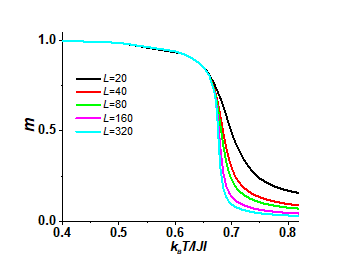
\includegraphics[width=\linewidth]{bab/image12.png}
        \caption{Температурная зависимость намагниченности $m$ для модели Поттса с $q=3$ на гексагональной решетке.}
        \label{fig:bab-2}
    \end{minipage}
    \hfill
    \begin{minipage}[c]{0.45\linewidth}
        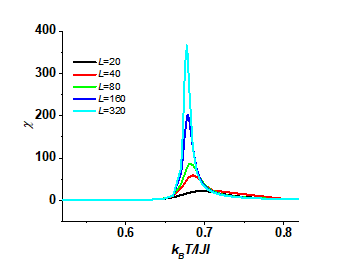
\includegraphics[width=\linewidth]{bab/image11.png}
        \caption{Температурная зависимость восприимчивости $\chi$ для модели Поттса с $q=3$ на гексагональной решетке.}
        \label{fig:bab-3}
    \end{minipage}
\end{figure}

На рисунках \ref{fig:bab-2} и \ref{fig:bab-3} представлены характерные зависимости намагниченности $m$ и 
восприимчивости $\chi$ для трехкомпонентной модели Поттса на гексагональной решетке от температуры соответственно. Здесь и далее на всех рисунках погрешность данных не превышает размеров символов, используемых для построения графиков. Как видно из этих рисунков, для всех рассмотренных систем наблюдается поведение характерное для фазового перехода второго рода.

В численных методах для определения температуры и рода ФП хорошо зарекомендовал себя метод кумулянтов Биндера четвертого порядка \cite{bib:bab-12}
\begin{gather}
    \label{eq:bab-6}
    V_L(T) = 1 - \frac{\left<E^4(T; L)\right>_L}{3\left<E^2(T; L)\right>_L^2}, \\
    \label{eq:bab-7}
    U_L(T) = 1 - \frac{\left<m^4\right>_L}{3\left<m^2\right>_{L^2}},
\end{gather}
где $E$ и $m$ -- энергия и намагниченность рассматриваемой системы с линейным размером $L$. Выражения \eqref{eq:bab-6} и \eqref{eq:bab-7} позволяют определить температуру $T_l$ фазового перехода с большой точностью в ФП первого и второго рода соответственно. Как известно ФП второго рода характеризуются следующими отличительными особенностями \cite{bib:bab-13}: усредненная величина $V_L(T)$ стремится к тривиальному значению $V^*$ согласно выражению
\begin{equation*}
    V(T) = V^* + bL^{-d}
\end{equation*}
при $L \to \infty$ и $T=T_c(L)$, где $V^* = 2/3$, а кумулянты Биндера $U_L(T)$ в критической области имеют четко выраженную точку пересечения. Указанные особенности для кумулянтов Биндера четвертого порядка $V_L(T)$ и $U_L(T)$ продемонстрированы на рис.~\ref{fig:bab-4} и \ref{fig:bab-5} соответственно для ферромагнитной трехкомпонентной модели Поттса на гексагональной решетке. Методика определения рода фазового перехода этим методом подробно описана в работе \cite{bib:bab-14}. Как видно из рис.~\ref{fig:bab-4} температура ФП в трехкомпонентной модели Поттса на гексагональной решетке $T_c=0.673(2)$. Следует отметить, что для двумерных моделей Поттса с числом состояний спина $q$ из соображений дуальности квадратной, треугольной и гексагональной решетки были получены простые полиномиальные выражения, позволяющие определить критическую температуру (см. \cite{bib:bab-8}). Однако эти выражения справедливы только для моделей Поттса с $q>3$ и $q=2$ \cite{bib:bab-9}.
\begin{figure}[ht]
    \begin{minipage}[c]{0.45\linewidth}
        \includegraphics[width=\linewidth]{bab/image18.png}
        \caption{Температурная зависимость кумулянтов Биндера $V_L(T)$ для трехкомпонентной модели Поттса на гексагональной решетке.}
        \label{fig:bab-4}
    \end{minipage}
    \hfill
    \begin{minipage}[c]{0.45\linewidth}
        \includegraphics[width=\linewidth]{bab/image17.png}
        \caption{Температурная зависимость кумулянтов Биндера $U_L(T)$ для трехкомпонентной модели Поттса на гексагональной решетке.}
        \label{fig:bab-5}
    \end{minipage}
\end{figure}

Для рассмотренной модели Поттса на гексагональной решетке нами исследовалось критическое поведение на основе применения теории конечно-размерного скейлинга (КРС). Из соотношений этой теории следует, что для достаточно большой системы с ПГУ при температуре $T=T_c$ намагниченность $m$, восприимчивость $\chi$ удовлетворяют следующим аналитическим выражениям \cite{bib:bab-15}
\begin{gather}
    \label{eq:bab-9}
    m \sim L^{-\beta / v}, \\
    \label{eq:bab-10}
    \chi \sim L^{\gamma / v}.
\end{gather}

Эти соотношения были нами использованы для определения $\beta / v$ и $\gamma / v$. Для аппроксимации температурной зависимости теплоемкости от $L$ использовалось выражение
\begin{equation}
    \label{eq:bab-11}
    C = A + BL^{\alpha / v},
\end{equation}
где $A$, $B$ -- некоторые коэффициенты.

В соответствии с теорией КРС в точке ФП для критического индекса радиуса корреляции $v$ выполняется соотношение \cite{bib:bab-16}
\begin{equation}
    \label{eq:bab-12}
    v_n = L^{\frac{1}{v}} g_{v_n},
\end{equation}
где $g_{v_n}$ -- некоторая постоянная, а в качестве $V_n$ могут выступать:
\begin{equation*}
    V_i = \frac{\left<m^i E\right>}{\left<m^i\right>} - \left<E\right>, \quad (i = 1, 2, 3).
\end{equation*}

Анализ данных, выполненный с использованием нелинейного метода наименьших квадратов, позволил определить значения $\beta / v$, $\gamma / v$, $\alpha / v$ и $1/v$ (см. Таблицу~\ref{tab:bab-1}). Затем, используя значения $v$, полученное в рамках данного исследования, определялись все остальные индексы $\beta$, $\gamma$, и $\alpha$. Точность критических индексов согласно выражениям теории КРС \eqref{eq:bab-9}-\eqref{eq:bab-12} в большей степени зависит от правильности учета данных для разных линейных размеров $L$. В наших расчетах строго контролировались данные для всех рассмотренных систем и при их незначительном отклонении от аппроксимирующей прямой процедура фитирования проводилась заново с отсеканием данных для $L<L_{\min}$. Такой отбор данных для разных линейных размеров $L$ позволяет заметно уменьшить погрешность в значениях КИ.
\begin{table}[ht]
    \centering
    \caption{Критические индексы для трехкомпонентной модели Поттса на гексагональной решетке}
    \label{tab:bab-1}
    \scriptsize
    \begin{tabular}{|p{2.4cm}*{9}{|c}|}
        \hline
        метод & $v$ & $1/v$ & $\alpha$ & $\alpha/v$ & $\gamma$ & $\gamma/v$ & $\beta$ & $\beta/v$ & $\alpha + 2\beta + \gamma = 2$ \\
        \hline
        Теория, \cite{bib:bab-9} & \makecell{5/6 \\ 0.83} & \makecell{6/5 \\ 1.20} & \makecell{1/3 \\ 0.333} & \makecell{2/5 \\ 0.40} & \makecell{13/9 \\ 1.444} & \makecell{26/15 \\ 1.733} & \makecell{1/9 \\ 0.111} & \makecell{2/15 \\ 0.133} & 2.0 \\
        \hline
        МК, гексагональная решетка (наши данные) & 0.847(3) & 1.180(2) & 0.327(3) & 0.387(3) & 1.446(1) & 1.708(3) & 0.107(3) & 0.127(3) & 1.99 \\
        \hline
        МК \cite{bib:bab-17}, квадратная решетка & & & & 0.46(8) & & 1.736(1) & & 0.131(1) & \\
        \hline
    \end{tabular}
\end{table} 